%                                             -*- coding: utf-8 -*-
% Mindenkinek csak javasolni tudjuk, hogy latex-et használjon.
% Szakdolgozatnál vagy diplománál már egyértelműen kijönnek az
% előnyei a Worddel szemben.  Ennek ellenére ez a sablon messze nem
% tökéletes.  Ha valamit javítanál benne, kérlek, küld vissza, hogy
% hallgatótársaid is profitáljanak belőle.  Köszönöm.

% További nehézséget okoz, hogy a népszerű latex disztribúciók nem
% tartalmazzák a legújabb változatát a magyar.ldf-nek.  A szükséges
% fájlokat a sablon mellé bemásoltuk, de le is tölthetőek innen:
% http://www.math.bme.hu/latex/
%
%
%
\documentclass[a4paper,oneside]{article}
\usepackage[margin=3cm]{geometry}
% =================================================================
% Magyar nyelvi támogatás
%------------------------
% ###################
% Nyelvváltó parancsok:
%\selectlanguage{english}
%\selectlanguage{magyar}
% rövid angol beszúrás:  \foreignlanguage{english}{some english text}
% határozott névelők generálása ``magyar'' babel-el:
% argumentum+megfelelő határozott nevelő: \az{},\Az{}
% csak a megfelelő határozott nevelő: \az*{}, \Az*{}
% címkék: \aref{}, \aref*{}, képletekhez \aref()
%        \Aref{}, \Aref*{}, képletekhez \Aref()
% oldalak: \apageref{}, \apageref*{}
%        \Apageref{}, \Apageref*{}
% idézetek: \acite, \acite*, \Acite, \Acite*
% ###################
\usepackage[english,magyar]{babel} %vegyes nyelvi támogatás a
% magyar helyesírás ellenőrzéshez (ispell) és elválasztáshoz
\selectlanguage{magyar}

%=================================================================
% direkt ékezetes karakter beírás támogatás
%-------------------------------------------
\usepackage[T1]{fontenc}
\usepackage[utf8]{inputenc}
\usepackage{multirow} 
%================================================================
% Undorító dolog bitmappelt (Type III) betűtípust nézni a PDF-ben
% képernyőn. Az alapértelmezett Computer Modern font LaTex-ben
% bitmappelt, ezért használjunk Times fontot:
\usepackage{times}

%================================================================
% ha ábrát akarunk beemelni, akkor használjuk a graphicx/graphics
% csomagot és az \includegraphics[width=<width>]{abra.pdf} parancsot
\usepackage{graphicx} %for graphics
%kepek helye a gyokerhez(ehhez a file-hoz kepest) kepest
\graphicspath{{./figs/}}

%================================================================
% Kötelezően használjuk a hyperref csomagot, mert ezzel többek között 
%  kultúrált hyperlinkelt PDF-et lehet csinálni az alábbi
%  variációkban, különféle hyperref backend-ekkel:
%  pdflatex,dvipdfm,ps2pdf
% tapsztalataim szerint a MikTeX (Win32) a 'dvipdfm' konverzióval
% optimális  míg a teTeX (Linux/Solaris) jobb szereti a 'dvips' módszert
%------------------------------------
% pontosan egyet kommentezzünk be!!!!!!!
% értelemszerűen backend függően generáljunk dvi-ból PDF-et!!!
%------------------------------------
% A hyperref csomag az utolsó beolvasott csomag legyen, kivéve néhány
% problémás csomagot, pl. algorithm
%-----------
% ########################### FONTOS ###########################
% A hyperref hibásan működik a babel csomag 'magyar.ldf' fájljának
% 1.5-ös verziójánál korábbi változatával. 2004. februárjában a MikTeX
% és teTex disztribúciók még csak a v.1.4 verziót tartalmazták! A fájl
% aktuális verziója a BME Matematikai intézet LaTeX honlapjáról
% elérhető: http://www.math.bme.hu/latex/ 
% A lusták kedvéért a jelen sablon mellé is mellékelem:
% magyarlatex_0.01-2.tar.gz 
% ########################### FONTOS ###########################
%-----------
\usepackage[colorlinks=true]{hyperref}

\usepackage{float}
\usepackage{mathtools}
\DeclarePairedDelimiter\ceil{\lceil}{\rceil}
%%%%%%%%%%%%%%%%%%%%%%%%%%%%%%%%%%%%%%%%%%%%%%%%%%%%%%%%%%%%%%%%%%%
% Itt kezdődik maga a dokumentum
%%%%%%%%%%%%%%%%%%%%%%%%%%%%%%%%%%%%%%%%%%%%%%%%%%%%%%%%%%%%%%%%%%
\begin{document}
%%%%%%%%%%%%%%%%%%%%%%%%%%%%%%%%%%%%%%%%%%%%%%%%%%%%%%%%%%%%%%%%%%%
% Ezt ne piszkáld!!!!
%%%%%%%%%%%%%%%%%%%%%%%%%%%%%%%%%%%%%%%%%%%%%%%%%%%%%%%%%%%%%%%%%%%
\pagestyle{myheadings} % legyen fejléc 

\newcommand{\onlabcim}{
  \begin{center}
    \huge{\textbf{Önálló laboratórium beszámoló}}

    \small{Távközlési és Médiainformatikai Tanszék}
  \end{center}
} 

% Argumentumok: #1=Név, #2=Neptunkód, #3=szakirány, #4=email, #5 konzulens-1, #6 konzulens-1-email, #7 konzulens-2, #8 konzulens-2-email
\newcommand{\onlabszerzo}[8]{

\begin{center}
  \begin{tabular}{ r l }
  készítette: & \textbf{#1}  \\
              & \href{mailto:#4}{\textbf{#4}}  \\
  neptun-kód: & \textbf{\texttt{#2}}  \\
  ágazat:     & \textbf{#3}  \\
  konzulens: & \textbf{#5}  \\
             & \href{mailto:#6}{\textbf{#6}} \\
  konzulens: & \textbf{#7}  \\
             & \href{mailto:#8}{\textbf{#8}}  \\
  
  \end{tabular}
\end{center}

}

% % Argumentumok: #1=Név, #2=email
% \newcommand{\konzulens}[2]{
%   \noindent\textbf{Konzulens:} #1 
%   \newline\emph{Email cím:}\/ \href{mailto:#2}{#2}
%   \newline
% 
% }

% Argumentumok: #1=Tanév (xxxx/xx alakban, #2=félév (pont nélkül)
\newcommand{\tanevfelev}[2]{
  \large\noindent\textbf{Tanév:} #1. tanév, #2. félév
  \newline
}

% Argumentumok: #1=téma címe 
\newcommand{\feladatcim}[1]{
  \large\noindent\textbf{Téma címe: #1}
  \bigskip
}

% Argumentumok: #1=téma részletei 
\newcommand{\feladatmaga}[1]{
\large\noindent\textbf{Feladat:} 
  \newline
 #1
 \newline
 \smallskip
}

% A fejezetek közé beágyazott irod.jegyzék
\def\thebibliography#1{\renewcommand{%
\baselinestretch}{1}\subsection{A tanulm\'anyozott irodalom jegyz\'eke}\list
 {\small [\arabic{enumi}]}{\settowidth\labelwidth{[#1]}\leftmargin\labelwidth
 \advance\leftmargin\labelsep
 \usecounter{enumi}}
 \def\newblock{\small \hskip .11em plus .33em minus .07em}
 \sloppy\clubpenalty4000\widowpenalty4000
 \sfcode`\.=1000\relax}
\let\endthebibliography=\endlist%


%%% Local Variables: 
%%% mode: latex
%%% TeX-master: "template"
%%% End: 
 % Ez kell!!!
\markright{Reményi Gergely Márk (KPZH44)} % egyoldalas fejléc!!!
%--------------------------------------------------------------------
% fedlap
%--------------------------------------------------------------------
\begin{titlepage}
%bme logo 
 \begin{figure}[h]
    \centering
      
\includegraphics[width=12cm]{bme_logo}
  \label{fig:bme_logo}
  \end{figure}
  \thispagestyle{empty}
  %cím generálás
  \onlabcim

% \begin{center}
%   \begin{tabular}{ p{3cm} p{5cm} }
%   
%   Készítette: & Beszámoló Péter  \\
%   Neptun-kód: & BPOX43  \\
%   Ágazat: & Médiainformatika  \\
%   E-mail cím: & b.peter@onlab.hu  \\
%   Konzulens: & Dr. Péhádes István  \\
%   E-mail cím: & pehades@tmit.bme.hu  \\
%   Konzulens: & Doktor Andusz  \\
%   E-mail cím: & doktora@tmit.bme.hu  \\
%   
%   \end{tabular}
% \end{center}

 
  %\szerzo argumentumok: #1=Név, #2=Neptunkód, #3=szakirány, #4=email,#5 konzulens-1, #6 konzulens-1-email, #7 konzulens-2, #8 konzulens-2-email
  \onlabszerzo{Reményi Gergely Márk}{KPZH44}{Mérnökinformatikus szak}{gergo@gergo.city}{Maliosz Markosz}{maliosz@tmit.bme.hu}{Simon Csaba}{simon@tmit.bme.hu}
 
 
%\feladatcim argumentuma a feladat rövid, 1 soros címe
  \feladatcim{Skálázás Kubernetesben egyedi metrikák alapján} 

  %\feladatmaga argumentuma a feladat 1-2 bekezdésnyi ismertetése
  \feladatmaga{A hallgató feladata egyedi metrikák alapján történő horizontális skálázás vizsgálata Kubernetes környezetben.
              A hallgató a félév során megismerkedik a Horizontal Pod Autoscaler (HPA) technológiával, kiépíti és konfigurálja
              Kubernetesben az egyedi metrikákat létrehozó csővezetéket.}

 
  %\tanevfelev argumentumok:
  % #1=Tanév (xxxx/xx alakban), #2=félév (pont nélkül!)
  
  \tanevfelev{2020/2021}{II}
 
\end{titlepage} 

%==================================================================
\section{A laboratóriumi munka környezetének ismertetése,
     a munka előzményei és kiindulási állapota}
\label{sec:kornyezet}
% A munka  előzményei és kiindulási állapota
% \newpage
\subsection{Bevezető}
\label{sec:bevezeto}

A skálázás az egyik legkomplexebb és legfontosabb feladat (TODO:forrás) a
számítástechnikában. A beszámolóban be fogom mutatni a Kubernetes konténer alapú
alkalmazáskezelő rendszert és azokat a mechanizmusokat, amelyek  horizontális
skálázást lehetővé teszik erőforrás (CPU, memória) és egyedi metrikák alapján.

\Aref{secsec:kubernetes} fejezetben röviden bemutatom a Kubernetest, csak azokat
az elemeit kiemelve, amelyek a skálázás bemutatásához szükségesek.
\Aref{secsec:hpa} fejezetben részletesebben kifejtem a Kubernetesnek azt a
komponensét, amely a lehtővé teszi a horizontális skálázást.
\Aref{secsec:custom_metrics} fejezetben bemutatom annak a csővezetéknek az
elemeit, amelyekkel megoldottam azt, hogy a Kubernetes egyedi metrikák alapján
tudjon skálázódni. \Aref{secsec:k6} fejezetben bemutatom azt a terhelésgeneráló
eszközt, amivel a skálázódást teszteltem. Végül \aref{sec:az-elvegzett-munka}
fejezetben bemutatok egy CPU és egy egyedi metrikák alapján történő skálázást.

\subsection{Elméleti összefoglaló}

\subsubsection{Kubernetes}
\label{secsec:kubernetes}

A Kubernetes egy Google által fejlesztett konténer orchesztrációs rendszer
\cite{kubernetes}, amely programok telepítését, skálázását, terheléselosztását
és helyreállítását automatizálja. A Kubernetes konténer szinten operál, amelyek
virtuális gépekhez hasonlítanak, azonban közös operációs rendszert használnak. A
konténereknek külön fájlrendszerük, CPU, memória és processz névterük van, ezzel
leválaszthatók a hoszt operációs rendszerről, amivel szabadon mozgathatóak
lesznek operációs rendszerek között. A Kubernetes elosztott rendszer, a
konténereket klaszterben futtatja. Minden klaszterben kiválasztásra kerül egy
(vagy több) master node, amely egy olyan számítógép, amely az egész klaszter
állapotáért felel. A klaszterben lévő többi számítógép worker node, ezeken
futnak a konténerek.  Az alábbiakban bemutatom a Kubernetesnek azon
komponenseit, amelyek szükségesek a konténerek automatikus horizontális
skálázásának megvalósításához.

\paragraph{Control plane}

A control plane \cite{kubernetes-cp-and-node}, magyarul a vezérlési sík
komponensei olyan processzekből állnak, amelyek a Kubernetes klaszter master
node-ján futnak, és a klaszter állapotáért felelnek. Például elindítanak egy
konténert, ha a klaszterben futó konténerek száma nem egyezik a konfigurációban
megadott konténerek számával. A vezérlési sík az alábbi processzekből áll:

\subparagraph{kube-apiserver}

Elérhetővé teszi a Kubernetes API-t.

\subparagraph{etcd}

A klaszterről tárol információkat egy kulcs-érték adatbázisban.

\subparagraph{kube-scheduler}

Eldönti, hogy az újonnan létrehozott konténerek melyik node-ra legyenek ütemezve.

\subparagraph{kube-controller-manager}

Azért felel, hogy a konfigurációs fájlokban megadott állapot konzisztens legyen
a klaszter állapotával. Például konténereket hoz létre vagy töröl.

\paragraph{Node}

A node-okon \cite{kubernetes-cp-and-node} futnak a klaszterbe telepített
konténerek. Ehhez szükséges, hogy minden node-on legyen a konténer futtatását
lehetővé tevő runtime (pl. Docker vagy containerd), valamint az alábbi
processzek:

\subparagraph{kubelet} A node-on futó konténerek állapotáért felel. A control
plane utasításait követve biztosítja, hogy megfelelő számú egészséges konténer
fusson a node-on.

\subparagraph{Kube-proxy} Olyan hálózati beállításokért felel a node-on, amelyek
a klaszterből kimenő, klaszterbe bemenő és a klaszteren belüli kommunikációt
teszik lehetővé.

\paragraph{Podok, replicasetek és deploymentek}

A podok \cite{kubernetes-pods} Kubernetesben a legkisebb telepíthető számítási
egység. Egy podban egy vagy több, szorosan összekapcsolódó konténer lehet.

Minden podnak egyedi IP címe van, ami lehetővé teszi a podok közötti
kommunikációt. A podokban lévő konténerek közvetlenül nem érhetnek
el más konténereket, a kommunikáció mindig a podokon keresztül történik. Egy
podon belül lévő konténerek viszont tudnak kommunkálni egymással a helyi
hálózaton.

Egy replicaset \cite{kubernetes-replicaset} objektummal lehet megadni a pod
klaszterben futú másolatainak számát. \Aref{secsec:hpa} fejezetben bemutatott
Horizontal Pod Autoscaler ezt az objektumot változtatja meg, amikor skálázódást
hajt végre.

Kubernetesben nem szokás külön pod és replicaset objektumokat létrehozni,
helyettük egy deployment \cite{kubernetes-deployment} objektumban érdemes
definiálni a telepítés kívánt állapotát, vagyis azt, hogy milyen konténerek
kerüljenek a podokba, és a podok másolatának a számát. A deploymentek
segítségével áramvonalassá válik a konténerek telepítése, frissítése, skálázása,
leállítása és visszagörgetése korábbi verziókra.

\paragraph{Service}

Kubernetesben service \cite{kubernetes-service} objektumok segítségével lehet
podokak elérni a klaszteren belül és kívülről.  A service-k podokhoz rendelt
címkék (label \cite{kubernetes-labels}) alapján választják ki a hozzájuk tartozó
podokat, amelyek között terheléseloszlást végeznek. Service-ekre azért van
szükség, mert a podokhoz rendelt ip-címek nem biztosítanak megfelelő
rugalmasságot.

A service-eknek több típusa van:

\begin{itemize}
  \item ClusterIP: alapértelmezett service, csak a klaszteren belül érhető el.
  \item NodePort: minden node-on nyit egy portot, amin keresztül elérthetőek a
  podok.
  \item LoadBalancer: klaszteren kívüli (tipikusan felhő) terheléselosztóján
  teszi elérhetővé a service-t.
\end{itemize}


\subsubsection{Horizontal Pod Autoscaler}
\label{secsec:hpa}

A horizontal pod autoscaler \cite{kubernetes-hpa} (HPA) objektum segítségével
lehet a podok számát skálázni Kubernetesben. A HPA alapértelmezetten tud cpu és
memória metrikák alapján skálázódni, egyedi metrikák alapján történő skálázás
körülményesebb, ezt \aref{secsec:custom_scaling} fejezetben mutatom be.

A HPA az alábbi képlettel számolja ki a kívánt replikák számát:
 
\begin{equation}
  kivantreplikak = \ceil{jelenlegireplikak * \frac{jelenlegimetrikaerteke }{kivantmetrikaerteke}}
\end{equation}


\subsubsection{Skálázás egyedi metrikák alapján}
\label{secsec:custom_metrics}

A Google nem gondoz az egyedi metrikák alapján történő skálázásról kiterjedt
dokumentációt, azonban újságcikkek alapján \cite{custom-metrics-1}
\cite{custom-metrics-2} fel lehet építeni egy olyan csővezetéket, amely begyűjti
a podok által generált metrikákat, és elérhetővé teszi a Kubernetes custom
metrics API-ja számára.

A legkézenfekvőbb megoldás Prometheus-t \cite{prometheus} használni a metrikák
begyűjtétéhez, és Prometheus Adaptert \cite{promehteus-adapter} használni a
begyűjtött adatok átalakítására a custom metrics API számára.
\Aref{fig:custom-metrics} ábrán látható az a csővezeték, amelyen keresztül az
egyedi metrikus adatoknak át kell menniük, hogy a HPA használni tudja őket.

\begin{figure}[H]
  \centering
  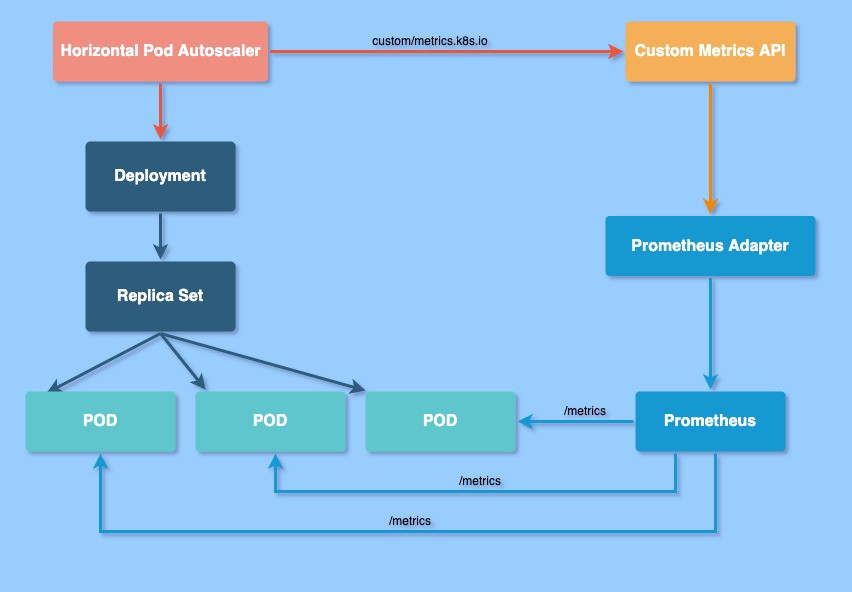
\includegraphics[width=\textwidth]{custom-metrics-pipeline.jpeg}
  \caption{Egyedi metrikák csővezetéke}
  \label{fig:custom-metrics}  
\end{figure}

A Prometheus nyílt forráskódú monitorozó és riasztó rendszer. Az idősoros
adatokat a \emph{/metrics} végpontról gyűjti be a pull modell szerint az
alkalmazásoktól, amiket PromQL \cite{promql} lekérdezőnyelvvel lehet lekérni. 

A Prometheus telepítése Kubernetesbe a legegyszerűbben egy operátor
\cite{operator} telepítésével végezhető. Kubernetesben az operátorok olyan
alkalmazáscsomagok, amelyek automatizálják egy adott alkalmazás karbantartását.
Mivel egy operátor sok komponensből áll, ezért célszerű Helmmel \cite{helm}
telepíteni, ami egy csomagkezelő a Kuberneteshez. 

A Promehteus pull modell szerint a \emph{/metrics} végpontokról gyűjti be a
metrikus adatokat. A végpontok felfedezéséhez a Prometheus operátor
\emph{ServiceMonitor} nevű custom resource-t \cite{custom-resource} definiál.
Ebben meg kell adni a monitorozni kívánt podok címkéjét és portját, ahol a
\emph{/metrics} végpont elérhető.

A Prometheus operátor alapértelmezetten tartalmazza a Grafana \cite{grafana}
nevű vizualizációs szoftvert, amelynek segítségével PromQL nyelven
lekérdezhetőek és vizualizálhatóak a Prometheus által gyűjtött metrikák.
\Aref{sec:az-elvegzett-munka} fejezetben szereplő ábrákat Grafanában hoztam
létre.

A Prometheus által gyűjtött metrikákat a Prometheus Adapter alakítja át a
Kubernetes custom metrics API-ja számára. Az adapter konfigurációja
\cite{prometheus-adapter-config} a következőképpen történik: 

\begin{itemize}
  \item Felfedezés: egy lekérdezés sablonját kell megadni, ami összegyűjti, hogy
  milyen objektumokon lehet a lekérdezést elvégezni
  \item Hozzárendelés: a felfedezésben begyűjtött objektumokat kell
  hozzárendelni Kubernetes erőforrásokhoz
  \item Megnevezés: meg kell adni a custom metrics API számára a metrika nevét
  \item Lekérdezés: meg kell adni, hogy maga a lekérdezés hogyan történjen
\end{itemize}

\subsubsection{Terhelésgenerálás K6-al}
\label{secsec:k6}

A mérések elvégzéséhez k6 \cite{k6} nevű terhelésgeneráló alkalmazást
választottam. Számomra az tette vonzóvá a k6-ot, hogy egy aktív közösség és
vállalat áll mögötte.

A k6-nak is van Kubernetes operátor csomagja \cite{k6-operator}, Bár még
kísérleti fázisban van, ennek ellenére (egy-két kisebb hibán kívül) jól
használható elosztott terhelési tesztek futtatására.

Az operátor jelenlegi állapotában a tesztet szigorúan egy \emph{test.js}-nek
elnevezett fájlban kell definiálni, ezután configmapként telepíteni kell a
klaszterbe. A tesztet egy k6 típusú custom resource létrehozásával lehet
elindítani. Ebben meg kell adni a configmap nevét, azt, hogy mennyi pod futtassa
a teszteket és hogy futhassanak-e a podok külön node-okon. A podok létrehozása
után még nem indul el a teszt, az összes k6 által létrehozott podon el kell
indítani a teszteket a \verb|k6 resume| paranccsal.
  
\newpage
%==================================================================
\section{Mérések elvégzése}
\label{sec:az-elvegzett-munka}

\subsection{Mérésekhez beállított alapértelmezett értékek}

A minden mérés elvégzéséhez egyetlen k6 tesztet definiáltam. Ebben a tesztben a
kapcsolatot kialakító virtuális felhasználók száma 10 perc alatt lineárisan
növekedik 0-tól 100-ig, majd 30 másodperc alatt visszaesik 0-ra. Minden
virtuális felhasználó egytized másodpercenként küld el egy HTTP GET kérést a
skálázandó podoknak.

A podokat úgy állítottam be, hogy 300 millicore legyen a limitjük, vagyis a node
CPU-jának maximum $3/10$-ad számítási kapacitását használhatják. A podoknak még
megadtam azt is, hogy csak olyan node-okon indulhatnak el, amelyeken van még 100
millicore-nyi szabad kapacitás.

\subsection{CPU alapú skálázás rövid válaszidejű végponton}
\label{secsec:cpu_scaling}

A CPU alapú skálázáshoz úgy állítottam be a HPA-t, hogy átlagosan 50\% alatt
maradjon a podok CPU igénye. Ez az 50\%-os küszöb a podok CPU limitjéhez
viszonyítva értelmezendő, vagyis ha egy pod korlátja 300 millicore, akkor a HPA
feladata lesz annyi új podot indítani, hogy a podok átlagos CPU erőforrás igénye
150 millicore alatt maradjon.

A teszt lefutásához négy diagramot hoztam létre Grafanában, amelyek szükségesek
a CPU alapú skálázás vizsgálatához és értékeléséhez, és amellyel össze lehet
vetni az egyedi metrikák alapján skálázódó teszt lefutásának adatait.


\Aref{light_cpu_hpa} ábrán láthatóak a HPA által kívánt podok száma (desired
replicas) és a podok tényleges száma (current replicas).  Az ábrán csak egy
adatsor látszik, mivel a két metrika együtt mozog.  Az ábrán látható az is, hogy
a HPA nem skálázza le a podokat egyből, hanem kivárja az alapértelmezetten
beállított 5 perces lehűlési időt.

\begin{figure}[H]
  \centering
  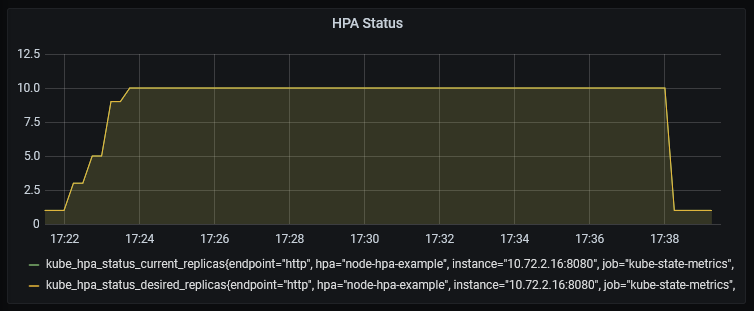
\includegraphics[width=\textwidth]{light_cpu_hpa.PNG}
  \caption{HPA által kívánt és tényleges podok száma CPU alapú skálázás esetén}
  \label{light_cpu_hpa}  
\end{figure}

\Aref{light_cpu_cpu} ábrán látható a skálázott podok CPU kihasználtsága.  A kék
színű grafikon jelöli az összes pod CPU kihasználtságát, a többi ugyanezt
podokra levetítve.  Az ábráról leolvasható, hogy a teljes CPU kihasználtság
maximuma 1250m.  Ezt leosztva a replikák számával, vagyis 10-el, 125m-et
kapunk, azaz a HPA jól működött, mert az átlagos CPU kihasználtság nem ment
150m fölé. Azonban egyenként megvizsgálva a podok CPU használatát, vannak
olyan podok, amelyek elérik, és sokáig a 300m-es tartományban maradnak, és
olyanok, amelyek a 100m-es tartományban maradnak.  Ebből látható, hogy a
Kubernetesben a terheléselosztás nem egyenletesen történik a podok között.

\begin{figure}[H]
  \centering
  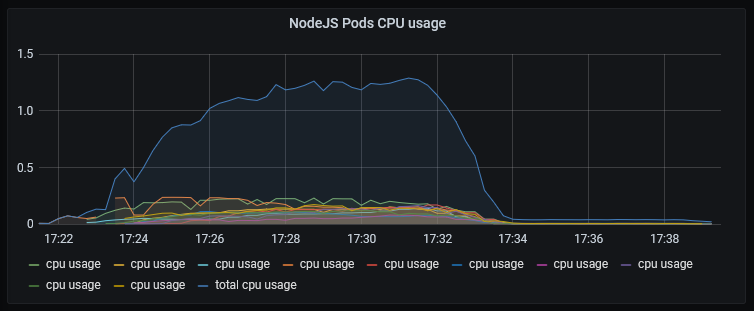
\includegraphics[width=\textwidth]{light_cpu_cpu.PNG}
  \caption{Kiszolgáló podok CPU kihaszáltsága}
  \label{light_cpu_cpu}  
\end{figure}

\Aref{light_cpu_response_time} ábrán az átlagos válaszidő látható podokra
bontva.  Kezdetben a podok jelentős része magasabb válaszidővel válaszol, ez
lehet a NodeJS Express valamilyen sajátossága miatt.  A válaszidők a teszt
közepe felé egyforma értékeket vesznek fel, majd kettő pod kivételével az összes
pod válaszideje megnő.  Ennek az lehet az oka, hogy a terhelésgenerálás olyan
fázisba ért, ahol a kéréseket a podok nem tudják azonnal kiszolgálni.

\begin{figure}[H]
  \centering
  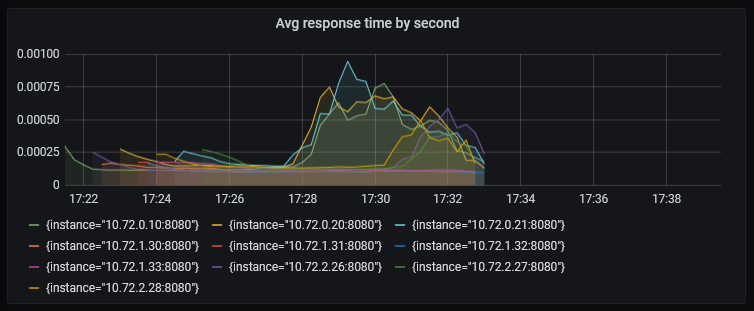
\includegraphics[width=\textwidth]{light_cpu_response_time.PNG}
  \caption{Kiszolgáló podok válaszideje 1 másodpercre vetítve}
  \label{light_cpu_response_time}  
\end{figure}

\Aref{light_cpu_response_count} ábrán az átlagos válaszok száma látható.  A zöld
színű grafikon jelöli az összes pod átlagos válaszainak számát.  Ez az ábra a
teszt szerint elvárt módon növekszik a 17:28-as időpontig, majd a válaszok
arányában stagnáció áll be.  \Aref{light_cpu_response_time} ábrával összevetve
arra lehet következtetni, hogy a stagnáció a podokra nehezedő terhelés
következménye.

\begin{figure}[H]
  \centering
  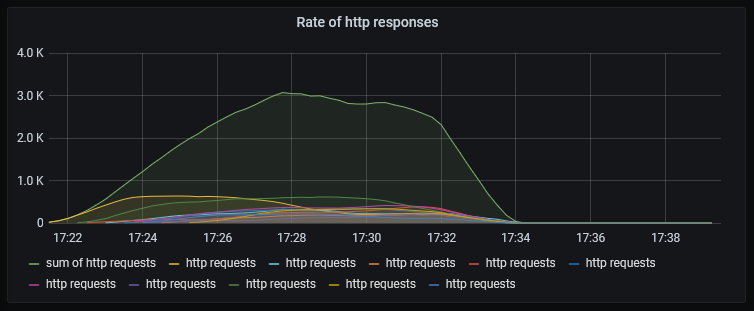
\includegraphics[width=\textwidth]{light_cpu_response_count.PNG}
  \caption{Kiszolgáló podok válaszainak száma 1 másodpercre vetítve}
  \label{light_cpu_response_count}  
\end{figure}

\subsection{Skálázás az átlagos válaszok számának függvényében}
\label{secsec:custom_scaling}

Az egyedi metrikára az átlagos válaszok számát választottam.  Az előző mérésből
\aref{light_cpu_response_count} ábra alapján az átlagos válaszok számának
küszöbét a HPA-ban 500-ra állítottam.

A teszt értékeléséhez ugyanolyan jellegű  ábrákat hoztam létre, mint a CPU alapú
skálázásnál \aref{secsec:cpu_scaling} fejezetben.

\Aref{light_custom_hpa} ábrán a HPA által kívánt és tényleges podok száma
látható.  Összevetve \aref{light_cpu_hpa} ábrával a podok száma sokkal lassabban
növekszik, és csak hat podot használ ki a maximális tízből.

\begin{figure}[H]
  \centering
  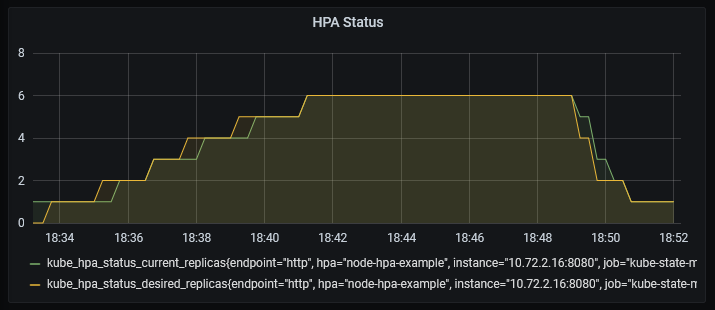
\includegraphics[width=\textwidth]{light_custom_hpa.PNG}
  \caption{HPA által kívánt és tényleges podok száma}
  \label{light_custom_hpa}  
\end{figure}

\Aref{light_custom_cpu} ábrán látható CPU kihasználtságot összevetve
\aref{light_cpu_cpu} ábrán látható CPU kihasználtsággal látható, hogy az egyéni
metrikákkal történő skálázásnál a CPU kihasználtság sokkal jobban követi a
tesztben is definiált lineáris terhelést, valamint a CPU terhelés kisebb, mint a
CPU alapú slálázás esetében.

\begin{figure}[H]
  \centering
  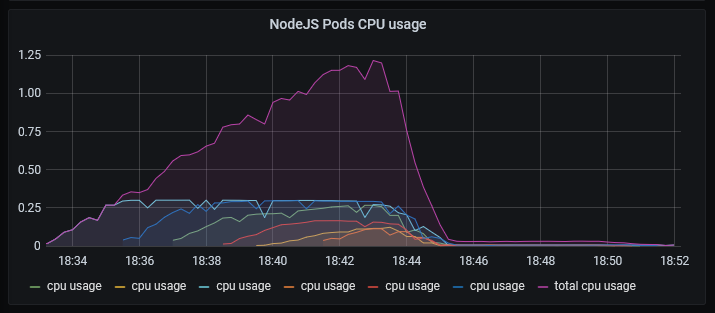
\includegraphics[width=\textwidth]{light_custom_cpu.PNG}
  \caption{Kiszolgáló podok CPU kihaszáltsága}
  \label{light_custom_cpu}  
\end{figure}

\Aref{light_custom_response_time} ábrán látható válaszidőket összevetve
\aref{light_cpu_response_time} ábrán látottakkal, a válaszidők a teszt elején
még jellegükben megegyeznek és az értékük is hasonló, a 0.1-0.2 ms tartományba
esik.  Az egyéni metrikákkal történő skálázásnál is megnőnek a válaszidők a
teszt végére,  azonban ez sokkal később történik meg, és csak két podnál (a
hatból) emelkedik számottevően.

\begin{figure}[H]
  \centering
  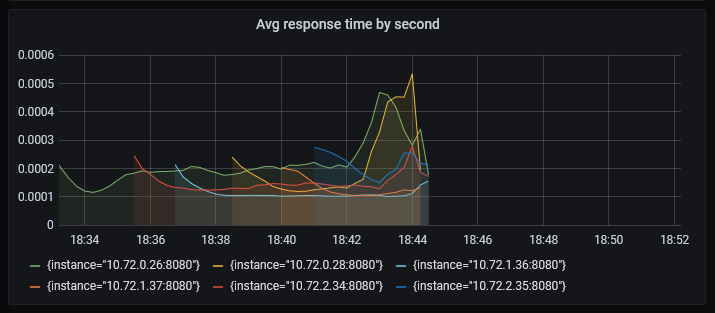
\includegraphics[width=\textwidth]{light_custom_response_time.PNG}
  \caption{Kiszolgáló podok válaszideje 1 másodpercre vetítve}
  \label{light_custom_response_time}  
\end{figure}

\Aref{light_custom_response_count} ábrán is megfigyelhető
\aref{light_custom_cpu} ábrához hasonló lineáris növekedés, azaz a válaszok
átlagos száma is jól követi a tesztben definiált terhelés növekedését.
Azonban itt is megfigyelhető, hogy mivel a HPA a podok válaszainak egy
másodpercre vetített számának átlagát veszi, a podok válaszainak száma nem
lesz 500 alá szorítva.

\begin{figure}[H]
  \centering
  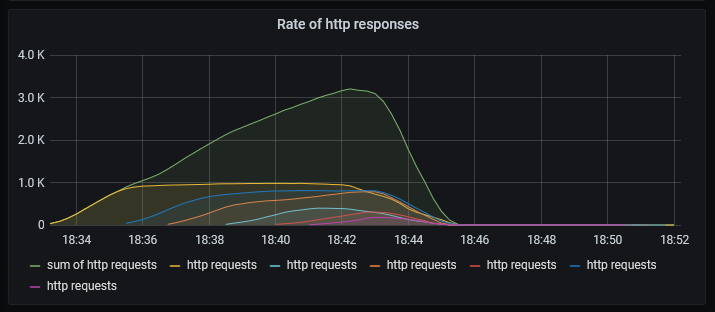
\includegraphics[width=\textwidth]{light_custom_response_count.PNG}
  \caption{Kiszolgáló podok válaszainak száma 1 másodpercre vetítve}
  \label{light_custom_response_count}  
\end{figure}

\subsection{Összefoglalás}
\label{sec:osszefoglalas}

\Aref{secsec:cpu_scaling} részben bemutattam egy CPU alapú skálázást és
\aref{secsec:custom_scaling} részben egy HTTP válaszok átlagos száma alapján
történő skálázást.  A tesztek futásakor kapott metrikák azt mutatták, hogy a
válaszok átlagos száma alapján történő skálázás CPU kihasználtságban és
válaszidőben is jobb eredményeket produkált, mint a CPU alapú skálázás.  A
mérésekből az a következtetés vonható le, hogy a tényleges terhelést leíró
metrikákat használva jobb kihasználtságot és jobb metrikus adatokat lehet kapni
az erőforrás alapú skálázáshoz képest.  A félév során a rendszer megismerésén és
a mérési környezet beállításán volt a fő hangsúly, de a következőkben a célom
gazdagabb szcenáriók kidolgozása és az eredmények alaposabb elemzése lesz.

\newpage
 
%==================================================================
\section{Irodalom, és csatlakozó dokumentumok jegyzéke}
\label{sec:irod-es-csatl}

\begin{thebibliography}{9}
\label{sec:tanulm-irod-jegyz}

\bibitem{kubernetes} \emph{What is Kubernetes?}
  \url{http://inflab.tmit.bme.hu/08o/lezar.shtml}, szerk.: Google,
  2021. február 1.

\bibitem{kubernetes-cp-and-node} \emph{Kubernetes Components}
  \url{https://kubernetes.io/docs/concepts/overview/components/}, szerk.: Google,
  2021. március 18.

\bibitem{kubernetes-pods} \emph{Pods}
  \url{https://kubernetes.io/docs/concepts/workloads/pods/}, szerk.: Google,
  2021. január 12.

\bibitem{kubernetes-replicaset} \emph{ReplicaSet}
  \url{https://kubernetes.io/docs/concepts/workloads/controllers/replicaset/}, szerk.: Google,
  2021. április 16.

\bibitem{kubernetes-deployment} \emph{Deployments}
  \url{https://kubernetes.io/docs/concepts/workloads/controllers/deployment/}, szerk.: Google,
  2021. február 11.

\bibitem{kubernetes-service} \emph{Service}
  \url{https://kubernetes.io/docs/concepts/services-networking/service/}, szerk.: Google,
  2021. április 23.

\bibitem{kubernetes-labels} \emph{Labels and Selectors}
  \url{https://kubernetes.io/docs/concepts/overview/working-with-objects/labels/}, szerk.: Google,
  2021. április 22.

\bibitem{kubernetes-hpa} \emph{Horizontal Pod Autoscaler}
  \url{https://kubernetes.io/docs/tasks/run-application/horizontal-pod-autoscale/}, szerk.: Google,
  2021. március 25.

\bibitem{custom-metrics-1} \emph{Kubernetes HPA with Custom Metrics from Prometheus}
  \url{https://towardsdatascience.com/kubernetes-hpa-with-custom-metrics-from-prometheus-9ffc201991e}, szerk.: Cezar Romaniuc,
  2021. június 26.
  
\bibitem{custom-metrics-2} \emph{Building Your Own Custom Metrics API for Kubernetes Horizontal Pod Autoscaler}
  \url{https://medium.com/swlh/building-your-own-custom-metrics-api-for-kubernetes-horizontal-pod-autoscaler-277473dea2c1}, szerk.: Cezar Romaniuc,
  2021. augusztus 31.

\bibitem{prometheus} \emph{Overview}
  \url{https://prometheus.io/docs/introduction/overview/}, szerk.:  Prometheus Authors,
  2018. december 13.

\bibitem{prometheus-adapters} \emph{Prometheus Adapter for Kubernetes Metrics APIs}
  \url{https://github.com/kubernetes-sigs/prometheus-adapter/blob/master/README.md}, szerk.:  Prometheus Adapter Authors,
  2020. november 6.

\bibitem{promql} \emph{Querying Promehteus}
  \url{https://prometheus.io/docs/prometheus/latest/querying/basics/}, szerk.: Prometheus Authors,
  2021. május 4.

\bibitem{operator} \emph{Operator pattern}
  \url{https://kubernetes.io/docs/concepts/extend-kubernetes/operator/}, szerk.: Google,
  2021. február 23.

\bibitem{helm} \emph{Using Helm}
  \url{https://helm.sh/docs/intro/using_helm/}, szerk.: Helm Authors,
  2021. május 4.

\bibitem{custom-resource} \emph{Custom Resources}
  \url{https://kubernetes.io/docs/concepts/extend-kubernetes/api-extension/custom-resources/}, szerk.: Google,
  2021. március 29.

\bibitem{grafana} \emph{Grafana basics}
  \url{https://grafana.com/docs/grafana/latest/basics/?pg=docs}, szerk.: Grafana Authors,
  2021. május 4.

\bibitem{prometheus-adapter-config} \emph{Configuration Walkthroughs}
  \url{https://grafana.com/docs/grafana/latest/basics/?pg=docs}, szerk.: Prometheus Adapter Authors,
  2020. október 28.

\bibitem{k6} \emph{What is k6?}
  \url{https://k6.io/docs/}, szerk.: k6 Authors,
  2020. május 4.

\bibitem{k6-operator} \emph{Running distributed k6 tests on Kubernetes}
  \url{https://k6.io/docs/}, szerk.: Simon Aronsson,
  2021. február 11.

\end{thebibliography}

%==================================================================
\subsection{A csatlakozó dokumentumok jegyzéke}
\label{sec:csat-irod}

\end{document} 

%%% Local Variables: 
%%% mode: latex 
%%% TeX-master: t 
%%% End:
